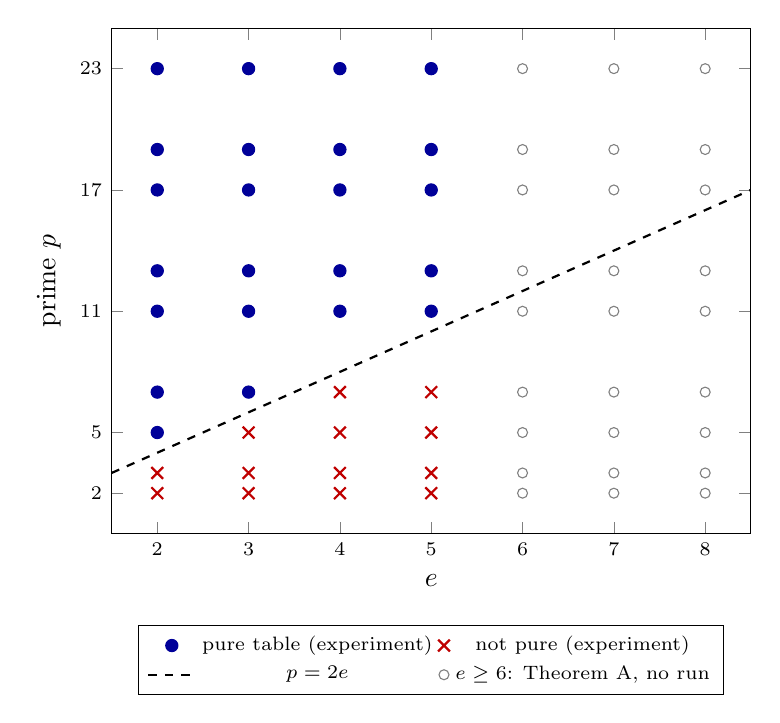
\begin{tikzpicture}
\begin{axis}[width=0.8\textwidth, height=8cm, xlabel={$e$}, ylabel={prime $p$}, xmin=1.5, xmax=8.5, ymin=0, ymax=25, xtick={2,...,8}, ytick={2,5,11,17,23}, tick label style={font=\scriptsize}, legend style={font=\scriptsize, at={(0.5,-0.18)}, anchor=north}, legend columns=2]
\addplot[only marks, mark=*, mark size=2.2pt, color=blue!60!black] coordinates {(2,5) (2,7) (2,11) (2,13) (2,17) (2,19) (2,23) (3,7) (3,11) (3,13) (3,17) (3,19) (3,23) (4,11) (4,13) (4,17) (4,19) (4,23) (5,11) (5,13) (5,17) (5,19) (5,23)};
\addlegendentry{pure table (experiment)}
\addplot[only marks, mark=x, mark size=3pt, thick, color=red!75!black] coordinates {(2,2) (2,3) (3,2) (3,3) (3,5) (4,2) (4,3) (4,5) (4,7) (5,2) (5,3) (5,5) (5,7)};
\addlegendentry{not pure (experiment)}
\addplot[dashed, thick, color=black] coordinates {(1.5,3) (8.5,17)};
\addlegendentry{$p=2e$}
\addplot[only marks, mark=o, mark size=1.8pt, color=gray] coordinates {(6,2) (6,3) (6,5) (6,7) (6,11) (6,13) (6,17) (6,19) (6,23) (7,2) (7,3) (7,5) (7,7) (7,11) (7,13) (7,17) (7,19) (7,23) (8,2) (8,3) (8,5) (8,7) (8,11) (8,13) (8,17) (8,19) (8,23)};
\addlegendentry{$e\ge 6$: Theorem A, no run}
\end{axis}
\end{tikzpicture}
